En el capítulo \ref{intro} hemos planteado el problema y una posible solución al mismo. El objetivo tanto del capítulo anterior como este es el de explicar los detalles de implementación de la solución que hemos propuesto.\par 
Si en el capítulo  \ref{arte} repasábamos el estado del arte y sentábamos las bases teóricas del proyecto, en este capítulo describiremos la tecnología de la que hacemos uso para ejecutar de solución que proponemos. Además justificaremos los motivos que nos han llevado a seleccionar esta tecnología y no otra.\par

\section{Dicom SR}\label{dicomSR}
En primer lugar hablaremos de la tecnología que nos impone el proyecto. Los PACs utilizan el estándar DICOM-SR y como nuestro objetivo es que la solución se integre en el ecosistema existente en los centros médicos deberemos emplear este estándar.\medskip\par

\subsection{Definición}
El estándar DICOM-SR se incluye dentro del suplemento 23 del estándar de imagen médica DICOM. Describe una arquitectura de documento que permite compartir, almacenar y transmitir información de informes médicos estructurados \cite{hussein2004dicom}.\par
Se diseñó con la intención de suplir la brecha entre la información contenida en las imágenes y la información que los profesionales médicos introducen en sus informes. Los ficheros DICOM-SR almacenan de forma no ambigua y jerárquica todos los conceptos que podemos encontrar en un informe médico tradicional y además pueden incluir referencias a:
\begin{itemize}
	\item Imágenes en formato DICOM. 
	\item Informes de estudios previos.
	\item Detalles de las imágenes.
\end{itemize}\par\medskip\par
El estándar define el modelo de la información y cómo debe gestionarse el documento, lo que permite personalizar muchos aspectos de la implementación final\cite{hussein2004dicom2}.\par
Sin embargo al tratarse de un estándar bastante complejo, han surgido soluciones bastante dispares, entre las que podemos encontrar:
\begin{itemize}
	\item Una implementación basada en la orientación objetos integrando el estándar DICOM-SR en la estructura de XML.\cite{tirado2002information}
	\item Una implementación extendiendo el modelo de objetos de documento XML (DOM).\cite{doi:10.1117}
	\item Una implementación en C y C++ del estándar. \cite{Riesmeier2001795}
\end{itemize}
\par
Desde la Asociación Nacional de Fabricantes eléctricos (NEMA), se están haciendo esfuerzos por unificar los criterios y seguir avanzando en la definición del estándar.\par
Para este proyecto se emplea una implementación en la que el informe se estructura en un XML. Expondremos los detalles de los ficheros DICOM-SR con los que trabajaremos en los apartados \ref{dicomsr:ficheros},\ref{dicomsr:plantillas}, \ref{dicomsr:vocabulario} y \ref{dicomsr:internacionalizacion}.\par

\subsection{Beneficios del estándar DICOM-SR}\label{dicom:beneficios}
A pesar de los problemas que surgen en la definición y en la implementación del estándar, los beneficios que aporta su desarrollo merecen el esfuerzo. Podemos encontrar un resumen exhaustivo de las ventajas de DICOM-SR en el siguiente artículo \cite{noumeir2006benefits}. Entre las mejoras que aporta a la práctica clínica más relevantes encontramos: 
\begin{itemize}
	\item Mejora la comunicación entre los profesionales, al utilizar un léxico estándar no hay lugar a traducciones o 	interpretaciones erróneas. 
	\item Los informes son más precisos y concisos. Los profesionales rellenan el informe utilizando los códigos adecuados sin 	las estructuras gramaticales que serían necesarias al redactar los informes de modo tradicional. 
	\item Se evitan los errores gramaticales y de transcripción.
	\item La interpretación de los informes es más sencilla y permite una interpretación asistida por ordenador. 
	\item Las imágenes DICOM y los informes DICOM-SR comparten la misma cabecera que contiene información acerca del paciente, 	lo que mejora el registro de información médica.
	\item El informe incluye medidas numéricas de las evidencias encontradas, que redundará en la precisión del informe.
	\item Permite ejecutar acciones automáticas sobre los informes permitiendo la minería de datos.
	\item Se enfatizan los contenidos. El informe en DICOM-SR no guarda información de cómo debe mostrarse al usuario.
	\item Permite la transformación a otros formatos. 
	\item Permite la integración con sistemas que reconozcan el habla. 
\end{itemize} 
Como podemos comprobar el desarrollo del estándar tiene un impacto beneficioso directamente sobre la práctica clínica, es por esto que en los últimos 5 años ha crecido el interés de la comunidad científica por explotar el estándar DICOM-SR.\par

\subsection{Estructura de un informe médico estructurado} \label{dicomsr:ficheros}
A continuación describiremos las características de un informe médico siguiendo el estándar DICOM-SR.\par
Un fichero DICOM-SR organiza el informe mediante contenedores \textit{<CONTAINER>}. Los contenedores no almacenan la información, únicamente la estructuran. Los contenedores tienen hijos \textit{<CHILDS>}, y es dentro de los hijos dónde se almacena la información correspondiente a un informe concreto. Cada elemento de información se agrupa con las etiquetas con el tipo del valor que designan el tipo de elemento que se almacena en el campo. En nuestro proyecto soportamos las siguientes:
\begin{itemize} 
 	\item \textit{<DATE>}: almacena fechas.
 	\item \textit{<TEXT>}: almacena texto sin formato.
 	\item \textit{<NUM>}: almacena enteros o boleanos.
 	\item \textit{<CODE>}: almacena campos multievaluados.
 \end{itemize}
Dentro de las secciones definidas por estas etiquetas de tipo valor dónde encontramos los datos del informe médico en pares de elementos clave-valor. Para designar la clave utilizamos la etiqueta \textit{<CONCEPT\_NAME>}, mientras que para referirnos al valor de este contenedor utilizamos la etiqueta \textit{<VALUE>}.
En el ejemplo de \ref{dicom-report-tags} podemos ver como se codifica el identificador \textit{M001} de una lesión de tipo masa. Vemos un contenedor que abarca el concepto \textit{masa} y entre los hijos encontramos el identificador de la masa que es de tipo texto.\par
En el campo valor, \textit{<VALUE>}, podremos encontrar:
\begin{itemize}
	\item Texto plano.
	\item Valores numéricos con sus unidades.
	\item Fechas.
	\item Imágenes DICOM.
	\item \ldots
\end{itemize}\par

Un punto importante para alcanzar los objetivos descritos en \ref{dicom:beneficios}, es trabajar con un léxico limitado y bien conocido, por lo que se utilizan diccionarios de conceptos médicos para identificar cada concepto de los que puede aparecer en un informe.Cada concepto del informe se identifica por su \textit{CONCEPT\_NAME} que está formado por tres en partes:
\begin{itemize}
	\item \textit{CODE\_SCHEMA}: identifica el diccionario dónde se encuentra el término que estamos definiendo.
	\item \textit{CODE\_VALUE}: es el código al término médico definido.
	\item \textit{CODE\_MEANING}: contiene una descripción en texto plano del término para que sea legible por el usuario.
\end{itemize}
La combinación de \textit{CODE\_SCHEMA} y \textit{CODE\_VALUE} identifica de modo único un concepto dentro del informe.\par
De nuevo empleando el ejemplo \ref{dicom-report-tags}, vemos que el concepto \textit{masa} se encuentra en el diccionario \textit{RADLEX} con el código \textit{RID3874}.\medskip\par

\lstset{escapechar=@,style=dicom}
\renewcommand*\lstlistingname{Código}
\begin{lstlisting}[label=dicom-report-tags,caption=Fragmento de un informe estructurado de una exploración de mama]
		  ...
          <CONTAINER>
            <CONCEPT_NAME>
              <CODE_VALUE>RID3874</CODE_VALUE>
              <CODE_SCHEMA>RADLEX</CODE_SCHEMA>
              <CODE_MEANING>Mass</CODE_MEANING>
            </CONCEPT_NAME>
            <CHILDS>
              <TEXT>
                <CONCEPT_NAME>
                  <CODE_VALUE>118522005</CODE_VALUE>
                  <CODE_SCHEMA>SNOMED-CT</CODE_SCHEMA>
                  <CODE_MEANING>Identifier</CODE_MEANING>
                </CONCEPT_NAME>
                <VALUE> M001 </VALUE>
              </TEXT>
              ...
\end{lstlisting}

La información DICOM-SR del informe rellena el árbol XML. Existen implementaciones del estándar que hacen uso de etiquetas específicas para indicar las relaciones entre los contenedores DICOM, pero debido a que los ficheros XML almacenan la información per se en forma de árbol estas etiquetas son redundantes.\par
En la figura \ref{fig:dicom-report} se puede ver un esquema del árbol de conceptos de un informe siguiendo el formato DICOM-SR. Se trata de un exploración de mama, en la que se ha encontrado una masa en la mama derecha y dos asimetrías en la mama izquierda. Los campos de tipo valor, es decir los atributos del contenedor padre los representamos utilizando los cuadrados grises. Mientras que los contenedores, que no almacenan información pero estructuran el informe, los representamos con los cuadrados magentas.\par
Podemos encontrar el fichero DICOM-SR completo del informe que representa esta figura en el apéndice \ref{dicom-sr}.	\par

\begin{figure}[ht]
\centering
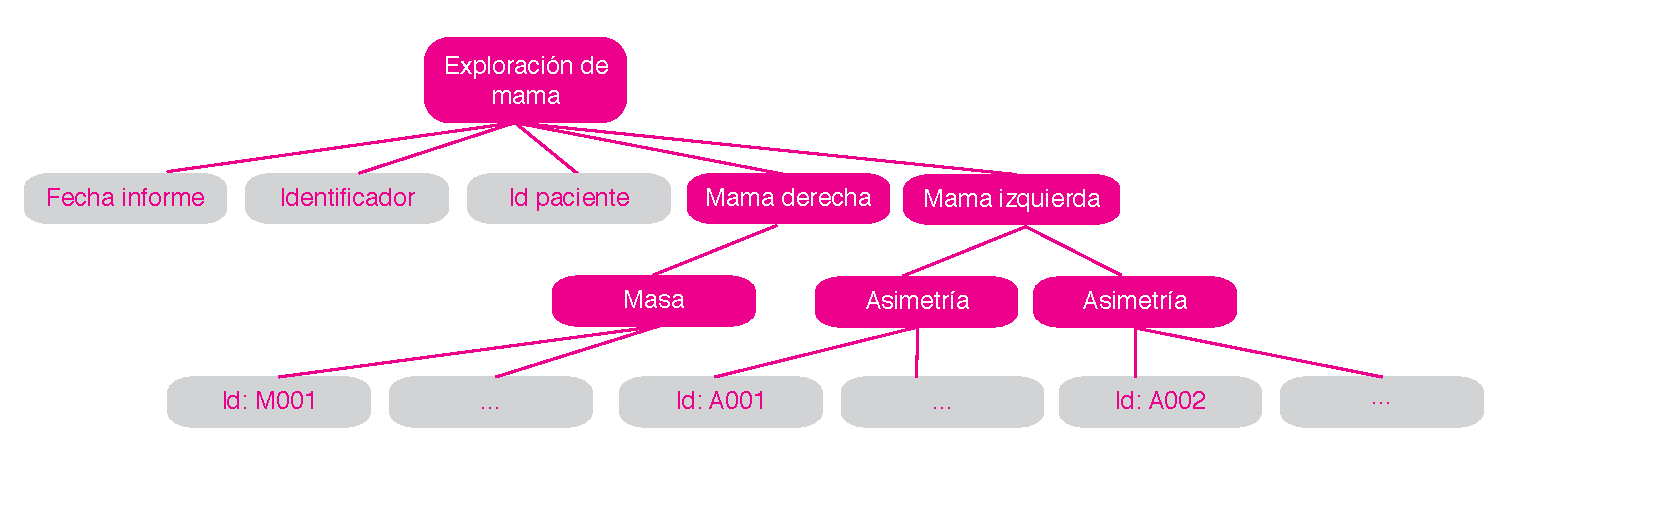
\includegraphics[scale=0.7]{./imgs/esquemas/dicomsrTreeReportA.pdf}
\caption{Representación del árbol XML de un informe en formato DICOM-SR}
\label{fig:dicom-report}
\end{figure}

\subsection{Estructura de una plantilla para un informe médico estructurado}\label{dicomsr:plantillas}
El estándar DICOM-SR, permite gran flexibilidad a la hora de escribir los informes estructurados. Esta característica puede complicarnos mucho el trabajo si cada especialista médico escribiera los informes siguiendo criterios correctos según el estándar pero aleatorios.\par
Para solucionar esto se crean las plantillas.\par
Las plantillas describen cómo debe ser un informe de tipo DICOM-SR, incluye los conceptos que debe tener así como las relaciones de jerarquía entre ellos y las propiedades que deben cumplir: si los conceptos son obligatorios o no, si pueden repetirse a lo largo del informe, \ldots\par 
Únicamente se guardan los conceptos en las plantillas, los campos correspondientes a los valores  \textit{<VALUE>} se incluirán después cuando el profesional rellene los datos para un paciente concreto.\par
El formato de las plantillas DICOM-SR es muy similar al de los informes DICOM. Carecen de las etiquetas \textit{<VALUE>} pero incluyen etiquetas \emph{<PROPERTIES>} para especificar las propiedades que deben tener los campos.\par
En el ejemplo \ref{dicom-template-mass} vemos como se almacenaría un concepto de tipo masa en una plantilla para la exploración de mama. Este contenedor podrá aparecer 0 o más veces en el informe final  (\textit{<CARDINALITY max=``-1'' min=``0''/>}) y lo introduce el usuario (\textit{<CONDITION\_TYPE type=``U''/>}).\medskip\par


\lstset{escapechar=@,style=dicom}
\renewcommand*\lstlistingname{Código}
\begin{lstlisting}[label=dicom-template-mass,caption=Fragmento de un plantilla informe estructurado: codificar una anomalía de tipo masa en una exploración de mama.]
		  ...
            <CONCEPT_NAME>
              <CODE_VALUE>RID3874</CODE_VALUE>
              <CODE_SCHEMA>RADLEX</CODE_SCHEMA>
              <CODE_MEANING>Mass</CODE_MEANING>
            </CONCEPT_NAME>
            <PROPERTIES>
              <CARDINALITY max="-1" min="0"/>
              <CONDITION_TYPE type="U"/>
              <EXPRESION_CONDITION xquery=""/>
            </PROPERTIES>
          ...
\end{lstlisting}

Además, en las plantillas de los contenedores se pueden incluir etiquetas para indicar la unidad de medida de los mismos, dentro de las etiquetas \emph{<UNIT\_MEASUREMENT>}. Estas etiquetas también servirán como modificadores como es el caso del ejemplo \ref{dicom-template-bool}, donde la etiqueta para el tipo del valor número, \textit{<NUM>}, se modifica de modo que el valor que introduzca el usuario será de tipo boleano, es decir sólo se permiten los valores 0 y 1. Así el concepto ``Cuadrante superior exterior de la mama derecha'' tendrá el valor verdadero o falso si la anomalía se sitúa en esa posición de la mama.\medskip\par

\lstset{escapechar=@,style=dicom}
\renewcommand*\lstlistingname{Código}
\begin{lstlisting}[label=dicom-template-bool,caption=Fragmento de una plantilla de un informe estructurado: codificar un atributo de tipo booleano.]
		  ...
              <NUM>
                <CONCEPT_NAME>
                  <CODE_VALUE>RID29929</CODE_VALUE>
                  <CODE_SCHEMA>RADLEX</CODE_SCHEMA>
                  <CODE_MEANING>Upper Outer Quadrant of Right Female Breast</CODE_MEANING>
                </CONCEPT_NAME>
                <PROPERTIES>
                  <CARDINALITY max="1" min="1"/>
                  <CONDITION_TYPE type="M"/>
                  <EXPRESION_CONDITION xquery=""/>
                  <DEFAULT_VALUE value="0"/>
                  <UNIT_MEASUREMENT>
                    <CONCEPT_NAME>
                      <CODE_VALUE>000000001</CODE_VALUE>
                      <CODE_SCHEMA>UNIT_MEASUREMENT</CODE_SCHEMA>
                      <CODE_MEANING>Boolean Units</CODE_MEANING>
                    </CONCEPT_NAME>
                  </UNIT_MEASUREMENT>
                </PROPERTIES>
              </NUM>
              ...
\end{lstlisting}

Las plantillas deben sintetizar el conocimiento de los especialistas técnicos que conozcan el estándar DICOM-SR y los profesionales médicos que conocen las características que deben tener los informes de las pruebas clínicas, por lo que será imprescindible la colaboración entre los profesionales de ambos ámbitos para crear las plantillas DICOM-SR.\medskip\par

Utilizamos estas plantillas como entrada para nuestro sistema. Tenemos una plantilla por ontología de exploración médica. Para este proyecto estamos trabajando con 4 ontologías diferentes.
\begin{itemize}
	\item Exploración de mama.
	\item Mamografía.
	\item Escáner de ultrasonidos.
	\item Resonancia Magnética
\end{itemize}

En el caso de las plantillas DICOM-SR la información también se estructura en forma de árbol. En el apéndice \ref{dicom-sr-template}, hemos incluido una plantilla truncada para el informe de una exploración de mama. En este apéndice se describe una plantilla que permite introducir lesiones de tipo masa en la mama derecha y asimetrías en la mama izquierda. El esquema \ref{fig:dicom-template} muestra esta plantilla con su  forma arbórea.\medskip\par

\begin{figure}[ht]
\centering
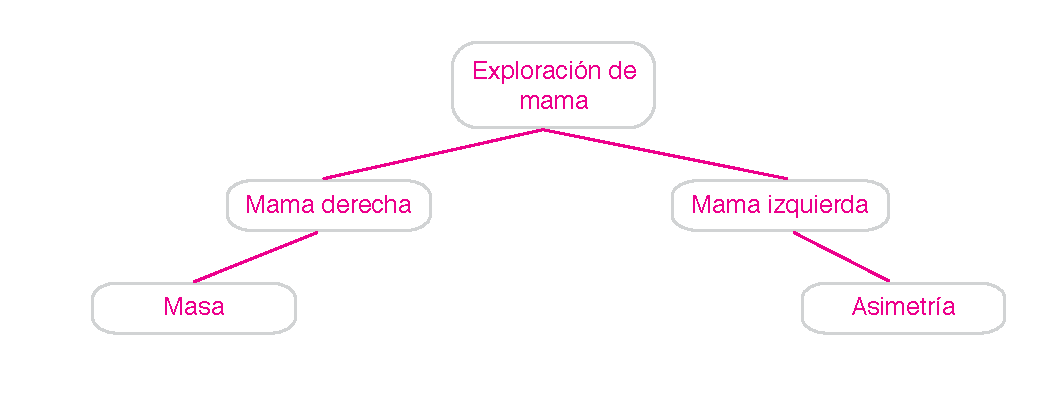
\includegraphics[scale=0.7]{./imgs/esquemas/dicomTreeTemplate.pdf}
\caption{Representación del árbol XML de una plantilla para un informe en formato DICOM-SR}
\label{fig:dicom-template}
\end{figure}


\subsection{Vocabulario}\label{dicomsr:vocabulario}
Un punto en el que hemos hecho hincapié es en la ventaja que supone que los informes hagan uso de un vocabulario estandarizado. Esto permite hacer referencia a conceptos concretos de manera precisa. Evitando los problemas que supone la barrera lingüística y la falta precisión del lenguaje natural.\medskip\par
También en lo que respecta al uso de vocabularios médicos DICOM-SR permite gran flexibilidad, permitiendo a los usuarios seleccionar el léxico que más les convenga en cada momento. En un mismo informe estructurado DICOM-SR pueden aparecer varios esquemas.\par
Los esquemas de codificación más habituales que podemos encontrar son: 
\begin{itemize}
	\item \emph{RadLex}: léxico desarrollado para cubrir las necesidades de la imagen radiológica. Contiene más de 30.000 términos. \cite{langlotz2006radlex}.
	\item \emph{ICD-10}: léxico generalista que contiene un índice internacional de enfermedades y problemas relacionados con la salud. Está traducido en 42 idiomas \cite{world2004icd}.
	\item \emph{SNOMED}: se considera la terminología clínica que más términos abarca y que soporta más lenguajes.\cite{stearns2001snomed} Se está convirtiendo en un estándar de facto al estar apoyado por numerosos gobiernos internacionales. \cite{snomed-gov}
\end{itemize}
\medskip\par
Sin embargo estos léxicos también presentan algunos inconvenientes: los conceptos pueden aparecer en varios léxicos, existen léxicos muy específicos para un país o idioma, no todos los léxicos se pueden integrar en DICOM-SR,\ldots\medskip\par
Para este proyecto utilizaremos los léxicos: \emph{RadLex}, \emph{SNOMED\-CT}, \emph{TRENCADIS\_MAMO} y \emph{UNIT\_MEASUREMENT}.\par
	
\subsection{Internacionalización}\label{dicomsr:internacionalizacion}
Las máquinas pueden trabajar con códigos como los que se almacenan en los léxicos médicos, incluso para algunas tareas puede ser incluso más beneficioso que tener que lidiar con secuencias de caracteres, especialmente si estos incluyen caracteres especiales. Pero las personas necesitamos el vocabulario para comprender los conceptos y poder trabajar con ellos.\medskip \par

La internacionalización y localización consiste precisamente en adaptar el software a los distintos idiomas y a las diferencias regionales como puedan ser los formatos de las divisas. No se trata únicamente de traducir las cadenas de texto.\par 
La internacionalización es la primera parte del proceso, consiste en diseñar y preparar el software que vamos a desarrollar y la localización es el proceso de adaptar el software creado a los distintos idiomas que se soporten.\cite{Uren:1993:ISI:562752}\medskip\par

Para presentar el informe para los profesionales médicos hacemos uso del texto codificado entre las etiquetas \emph{<CODE\_MEANING>}, sabiendo que algunos de los léxicos que se pueden incluir dentro un informe estructurado DICOM-SR están traducidos a múltiples idiomas, necesitamos encontrar una manera de que el significado del concepto sea diferente para cada lenguaje.\par
El estándar DICOM-SR especifica que las cadenas que se introduzcan en el campo \emph{<CODE\_MEANING>} pertenezcan al léxico con el que se esté trabajando, lo que no implica que estos textos deban estar en inglés, pero restringe la posibilidad de implementar soluciones en las que las traducciones no provengan de fuentes oficiales, porque esto nos conduciría de nuevo a la confusión semántica que pretendíamos evitar con el uso de vocabularios.\par
La solución que se propone en la literatura \cite{clunie2000dicom}, es hacer uso de la codificación del fichero para deducir que lenguaje del mismo, pero aunque se trata de una solución sencilla que no implica tener que trasmitir ni almacenar más información, como varios idiomas pueden utilizar la misma codificación no hay ninguna manera de diferenciarlos siguiendo este método. La otra solución que se propone es utilizar una etiqueta para identificar el idioma. Los ficheros DICOM-SR con los que trabajamos optan por la segunda opción. Utilizan la etiqueta \emph{<CODE\_MEANING>} para un primer idioma y \emph{<CODE\_MEANING2>} para un segundo como podemos ver en el ejemplo \ref{code-meaning}.\par

\lstset{escapechar=@,style=dicom}
\renewcommand*\lstlistingname{Código}
\begin{lstlisting}[label=code-meaning,caption=Internacionación y localización en ficheros DICOM-SR.]
		  ...
  <CONTAINER>
    <CONCEPT_NAME>
      <CODE_VALUE>RID10312</CODE_VALUE>
      <CODE_SCHEMA>RADLEX</CODE_SCHEMA>
      <CODE_MEANING>Resonancia Magnética</CODE_MEANING>
      <CODE_MEANING2>Magnetic Resonance Imaging</CODE_MEANING2>
    </CONCEPT_NAME>
              ...
\end{lstlisting}


En nuestro proyecto trabajaremos con plantillas localizadas para castellano e inglés como las que hemos visto en el ejemplo \ref{code-meaning}, así como con plantillas únicamente en inglés sin localizar como los fragmentos vistos en los ejemplos \ref{dicom-report-tags}, \ref{dicom-template-mass} y \ref{dicom-template-bool}

\section{Android}
Los teléfonos móviles inteligentes y las tabletas son tecnologías que ya llevan bastante tiempo entre nosotros, pero es en los últimos cinco años cuando la tecnología ha crecido exponencialmente. El índice de penetración en el mercado supera el 50\% en el caso de China y Estados Unidos, mientras que en Europa encontramos porcentajes inferiores, alrededor del 25\% pero las previsiones estiman que estas tasas crezcan rápidamente.\cite{wiki:smartphones}\par
La integración de dispositivos, la posibilidad de acceder a Internet y sobretodo la simplicidad de su uso fomentada por la posibilidad de interactuar con el dispositivo a través de la pantalla táctil, mucho más intuitivo que el teclado y el ratón, junto con un muy buen diseño de interfaces han facilitado la gran adopción de esta tecnología ya que han conseguido ampliar el espectro de usuarios potenciales\medskip\par

Un punto fundamental en el éxito de estas tecnologías es sin duda el nacimiento de Android.\par
Android es un sistema operativo basado en Linux, diseñado para trabajar con dispositivos móviles con pantallas táctiles. Fue desarrollado inicialmente por Android Inc., que fue comprada por Google en 2005. En el 2007 se forma la Open Handset Alliance: un conglomerado de empresas de hardware, software y telecomunicaciones cuyo objetivo es el de crear un entorno estandarizado para el desarrollo de dispositivos móviles. La OHA disponía de todos los agentes necesarios para revolucionar el mercado de las comunicaciones móviles y es en Octubre de 2008 cuando aparece el primer teléfono inteligente el HTC Dream que corría un Android 1.0.\cite{wiki:android}\medskip\par

A partir de este momento el desarrollo de Android no ha dejado de crecer, convirtiéndose en una tecnología clave.\par
Como ya se ha comentado en el apartado \ref{intro}, el uso de terminales móviles inteligentes en la práctica clínica para trabajar con imagen médica ha dado resultados muy satisfactorios. Por lo tanto, es obvio pensar que una aplicación para recopilar informes médicos sobre Android tendrá mejor acogida por parte del personal médico, ya que es más sencillo e intuitivo introducir los datos de los informes DICOM-SR. Y al facilitar esta tarea al personal médico, es más factible que podamos adquirir más informes DICOM-SR con los que realizar estudios posteriores.\par 

\subsection{Arquitectura}
En este apartado hablaremos brevemente de la arquitectura de Android.\par
Android es un sistema operativo abierto basado en Linux, cuyo núcleo está escrito en C y C++, y que fundamentalmente tiene soporte para Java. Google libera periódicamente el código del sistema operativo bajo la licencia Apache.\par 
\begin{figure}[ht]
\centering
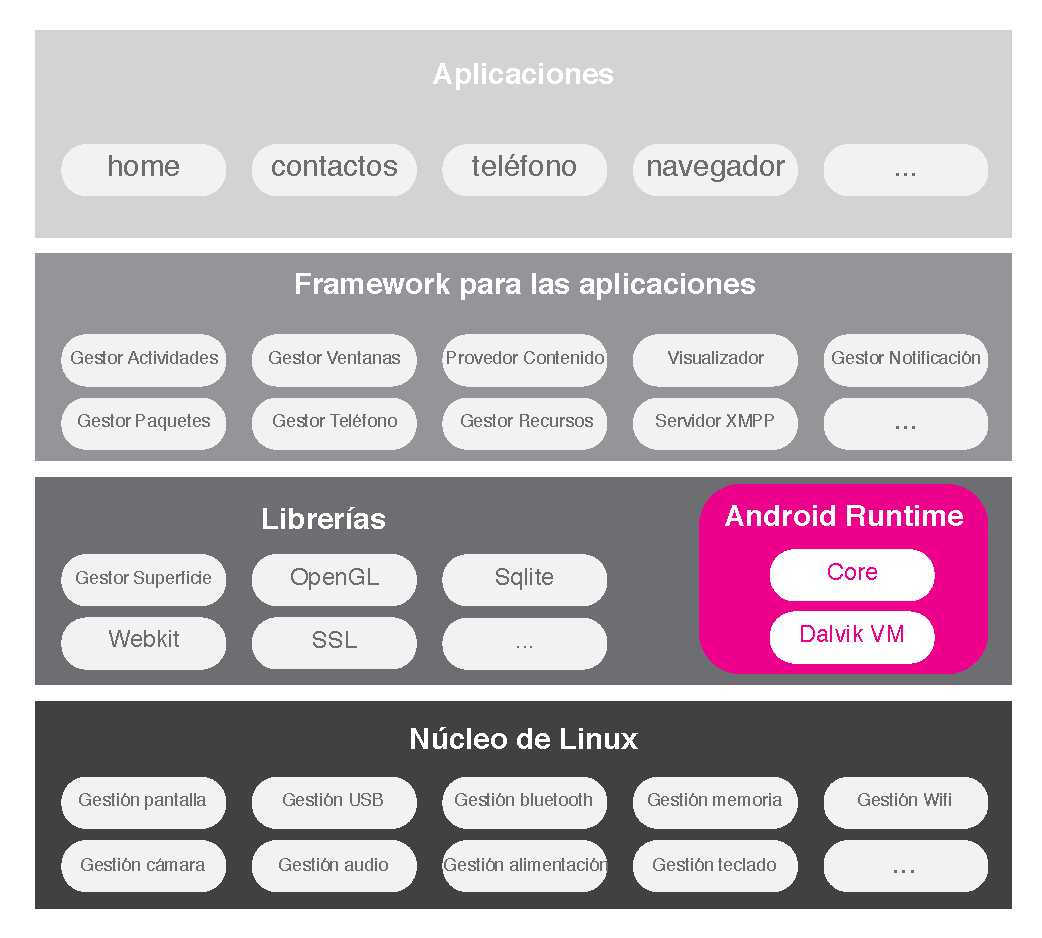
\includegraphics[scale=0.8]{./imgs/esquemas/arquitectura.pdf}
\caption{Arquitectura Android}
\label{fig:arquitectura_android}
\end{figure}

En la figura \ref{fig:arquitectura_android} vemos un esquema de la arquitectura Android, compuesta por:
\begin{itemize}
\item \emph{Núcleo Linux}: el núcleo es un fork el núcleo de la versión 2.6 de Linux. Sirve de abstracción con el hardware y gestiona los recursos del sistema. 
\item \emph{Librerías}: librerías nativas del sistema las utilizará el framework de Android para comunicarse con el hardware. Están escritas en C o C++.
\item \emph{Android Runtime}: se trata del entrono de ejecución de Android. Se integra con las librerías. Aquí tenemos el conjunto de librerías habituales de java, así como librerías Java específicas para Android. La Dalvik VM, es la máquina virtual de Java que ejecutará la aplicaciones. 
\item \emph{Framework para aplicaciones}: Capa formada por las clases y servicios que utilizan directamente las aplicaciones de usuario para interactuar con Android. 
\item \emph{Aplicaciones}: esta última capa incluye todas las aplicaciones del sistema y las instaladas por el usuario, tanto las nativas como las escritas en java.

\end{itemize}




\subsection{Segmentación}
La segmentación es uno de los problemas 


\subsection{Tabletas e interfaces táctiles de grandes dimensiones}

\section{Python}
